\chapter{Detailed Results}
\label{app:res}

\section{Simulation}
\label{app:sim}

\begin{table}[h]
\centering
\begin{tabular}{|c|c|c|c|} \hline
Simulation 		& reverberations 		& Added white noise at SNR [dB] 	& Standard deviation of position errors \\ \hline
1 				& Excluded  			& 60						 		& 0 \\
2 				& Included 				& 60						 		& 0 \\
3 				& Excluded  			& 40						 		& 0 \\
4 				& Included 				& 40						 		& 0 \\
5 				& Excluded 				& 60						 		& 0.05 \\
6 				& Included  			& 60						 		& 0.05 \\ \hline
\end{tabular}
\caption{The simulated scenarios}
\label{my-label}
\end{table}

\newpage



\subsection{Simulation 1}
\label{app:sim1}
\FloatBarrier
\begin{figure}[h!]
	\centering  
	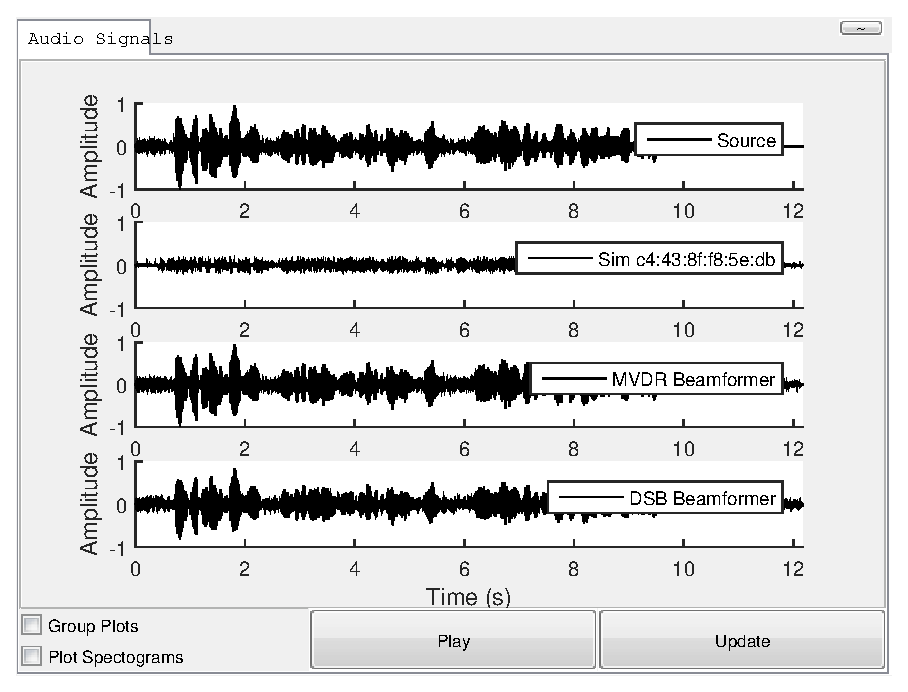
\includegraphics[scale = 0.9] {Screenshots_simulatie/Audio_signals/Signals_sim1} % l b r t]
	\caption[Audio signals simulation 1]{Audio signals simulation 1: Without reverberations, White noise added at 60dB SNR, without position errors} 
	\label{fig:Asim1}
\end{figure}

\begin{figure}[b!]
	\centering  
	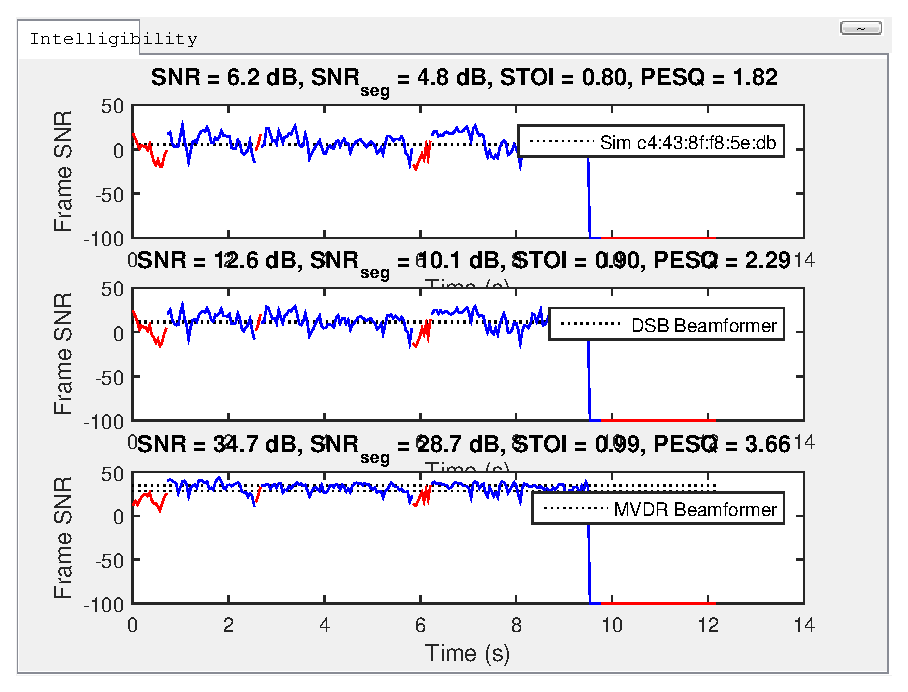
\includegraphics[scale = 0.9] {Screenshots_simulatie/Intelligibility/Simulatie1} % l b r t]
	\caption[Intelligibility simulation 1]{Intelligibility simulation 1: Without reverberations, White noise added at 60dB SNR, without position errors} 
	\label{fig:Isim1}
\end{figure}
\FloatBarrier
\subsection{Simulation 2}
\label{app:sim2}

\begin{figure}[h!]
	\centering  
	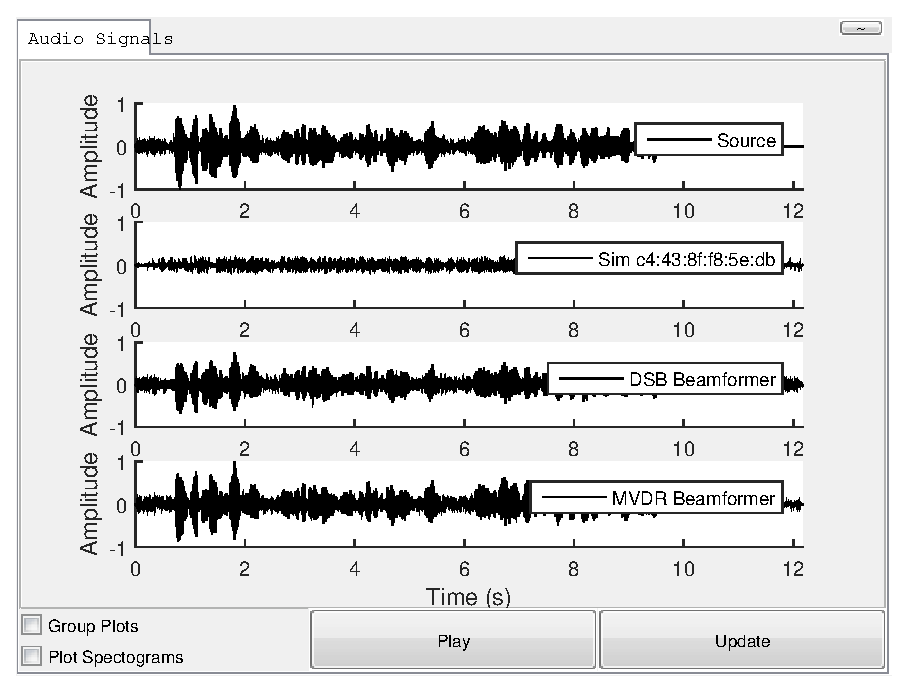
\includegraphics[scale = 0.9] {Screenshots_simulatie/Audio_signals/Signals_sim2} % l b r t]
	\caption[Audio signals simulation 2]{Audio signals simulation 2: With reverberations, White noise added at 60dB SNR, without position errors} 
	\label{fig:Asim2}
\end{figure}

\begin{figure}[b!]
	\centering  
	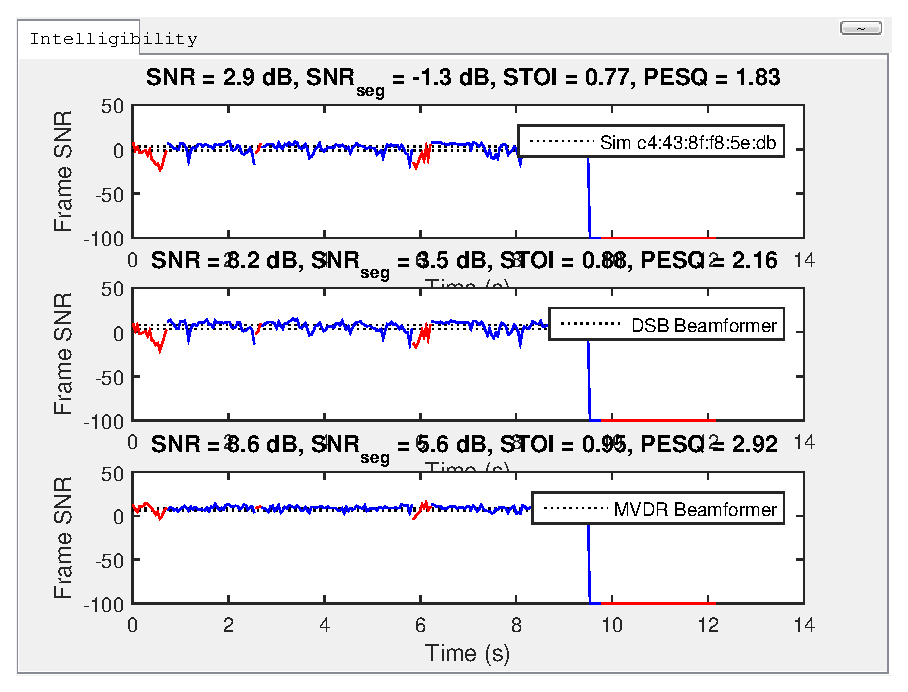
\includegraphics[scale = 0.9] {Screenshots_simulatie/Intelligibility/Simulatie2} % l b r t]
	\caption[Intelligibility simulation 2]{Intelligibility simulation 2: With reverberations, White noise added at 60dB SNR, without position errors} 
	\label{fig:Isim2}
\end{figure}
\FloatBarrier
\subsection{Simulation 3}
\label{app:sim3}

\begin{figure}[h!]
	\centering  
	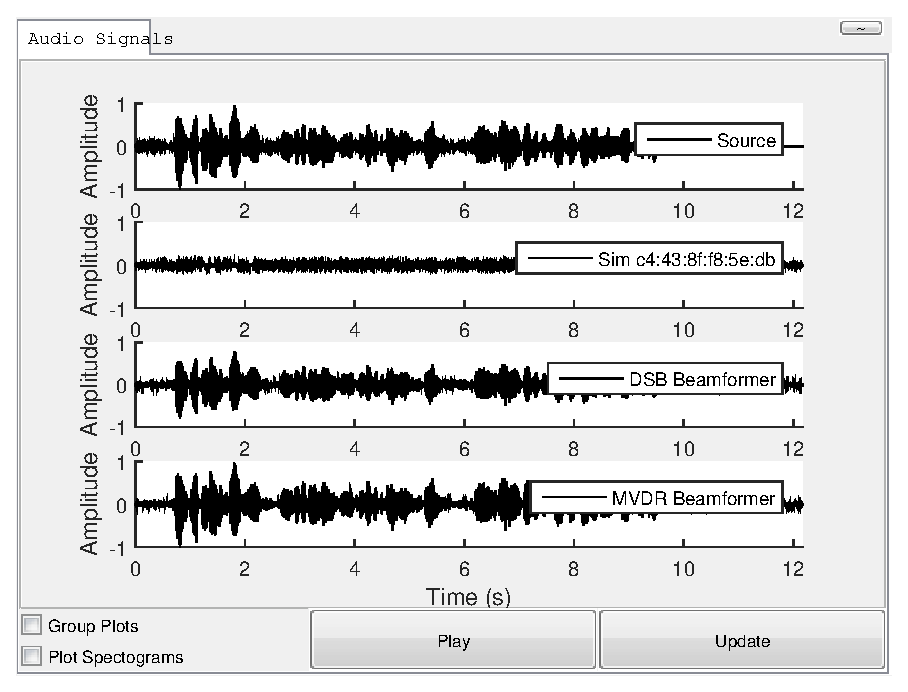
\includegraphics[scale = 0.9] {Screenshots_simulatie/Audio_signals/Signals_sim3} % l b r t]
	\caption[Audio signals simulation 3]{Audio signals simulation 3: Without reverberations, White noise added at 40dB SNR, without position errors} 
	\label{fig:Asim3}
\end{figure}

\begin{figure}[b!]
	\centering  
	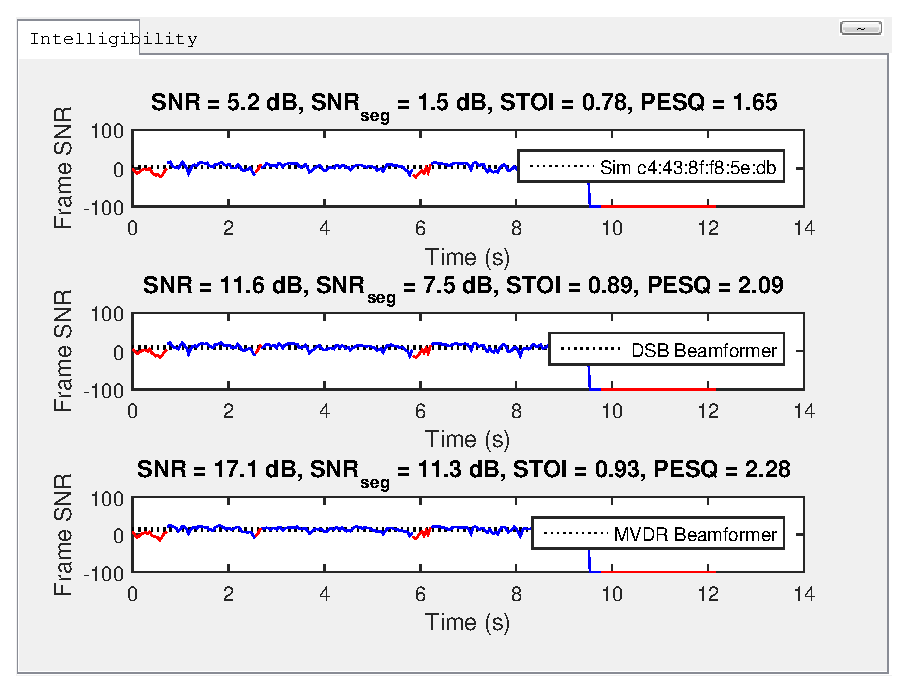
\includegraphics[scale = 0.9] {Screenshots_simulatie/Intelligibility/Simulatie3} % l b r t]
	\caption[Intelligibility simulation 3]{Intelligibility simulation 3: Without reverberations, White noise added at 40dB SNR, without position errors} 
	\label{fig:Isim3}
\end{figure}
\FloatBarrier
\subsection{Simulation 4}
\label{app:sim4}

\begin{figure}[h!]
	\centering  
	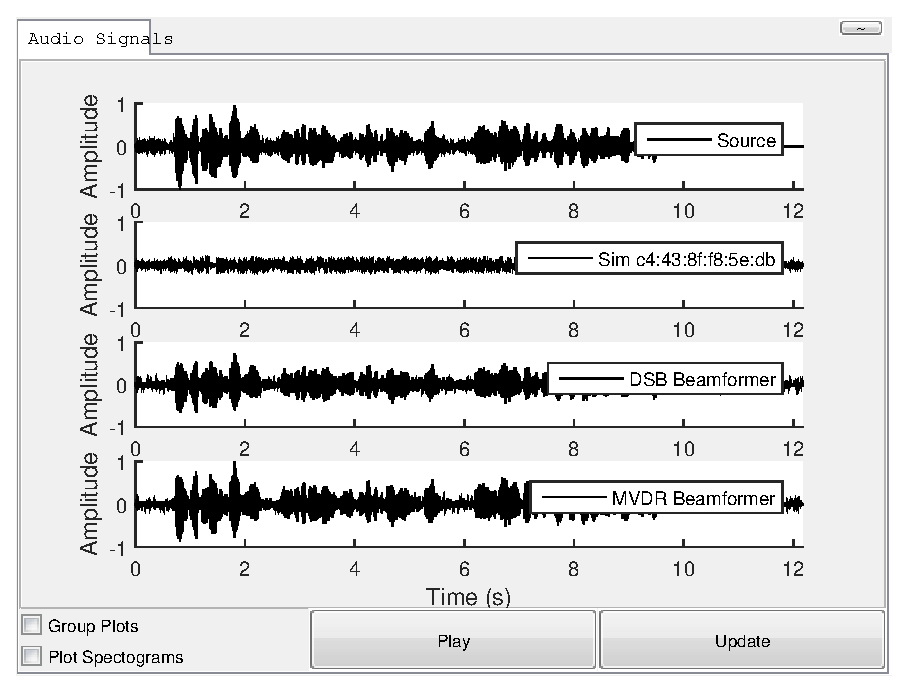
\includegraphics[scale = 0.9] {Screenshots_simulatie/Audio_signals/Signals_sim4} % l b r t]
	\caption[Audio signals simulation 4]{Audio signals simulation 4: Without reverberations, White noise added at 40dB SNR, without position errors} 
	\label{fig:Asim4}
\end{figure}

\begin{figure}[b!]
	\centering  
	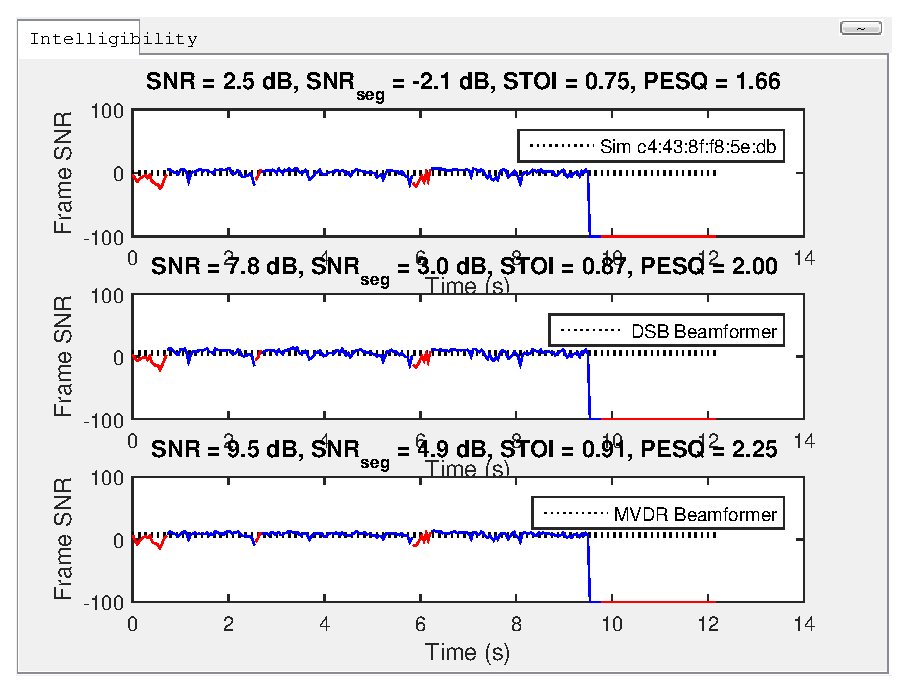
\includegraphics[scale = 0.9] {Screenshots_simulatie/Intelligibility/Simulatie4} % l b r t]
	\caption[Intelligibility simulation 4]{Intelligibility simulation 4: Without reverberations, White noise added at 40dB SNR, without position errors} 
	\label{fig:Isim4}
\end{figure}
\FloatBarrier
%\subsection{Simulation 5}
%\label{app:sim5}
%
%\begin{figure}[h!]
%	\centering  
%	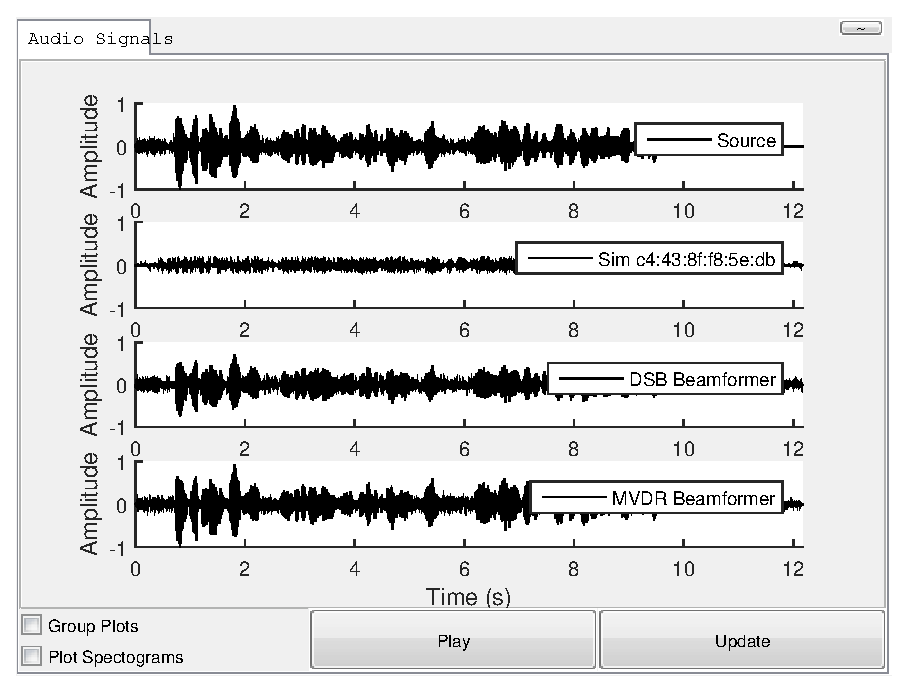
\includegraphics[scale = 0.9] {Screenshots_simulatie/Audio_signals/Signals_sim5} % l b r t]
%	\caption[Audio signals simulation 5: Without reverberations, White noise added at 60dB SNR, with position errors with a standard deviation of $0.05 cm$]{Audio signals simulation 5: Without reverberations, White noise added at 60dB SNR, with position errors with a standard deviation of $0.05 cm$} 
%	\label{fig:Asim5}
%\end{figure}
%
%\begin{figure}[b!]
%	\centering  
%	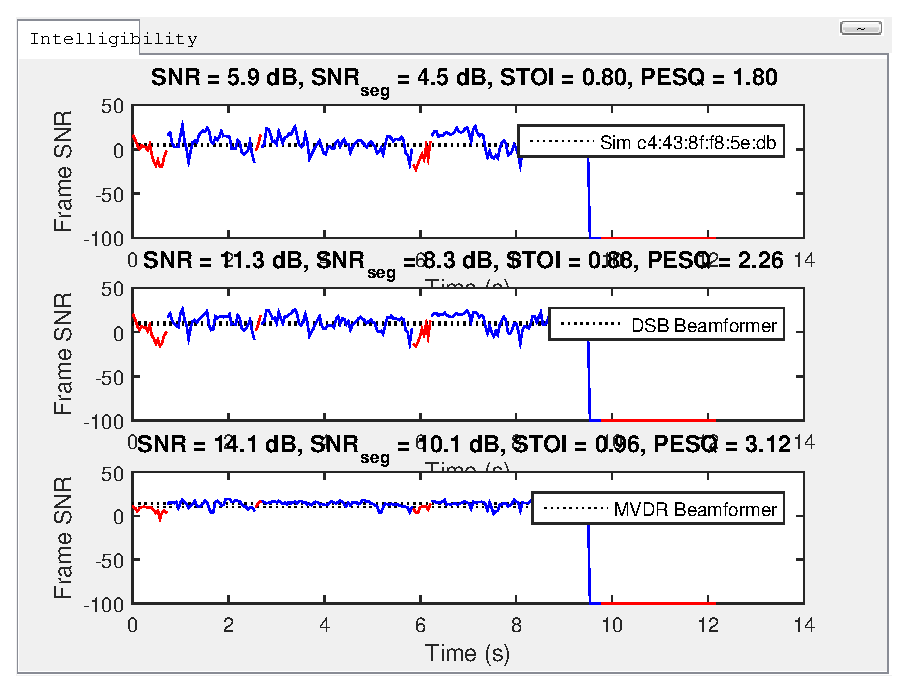
\includegraphics[scale = 0.9] {Screenshots_simulatie/Intelligibility/Simulatie5} % l b r t]
%	\caption[Intelligibility simulation 5: Without reverberations, White noise added at 60dB SNR, with position errors with a standard deviation of $0.05 cm$]{Intelligibility simulation 5: Without reverberations, White noise added at 60dB SNR, with position errors with a standard deviation of $0.05 cm$} 
%	\label{fig:Isim5}
%\end{figure}

\subsection{Simulation 6}
\label{app:sim6}

\begin{figure}[h!]
	\centering  
	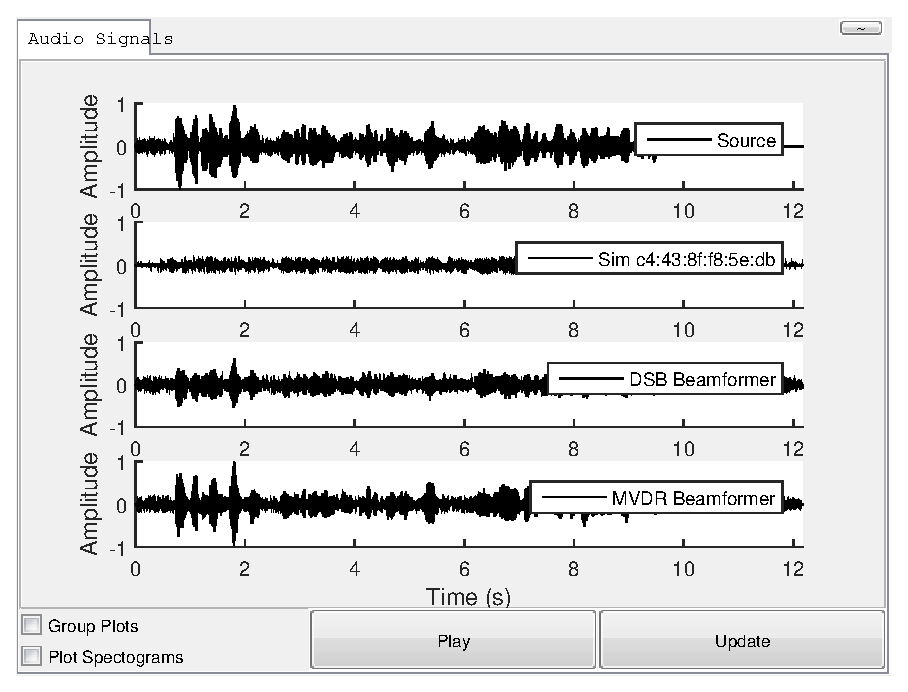
\includegraphics[scale = 0.88] {Screenshots_simulatie/Audio_signals/Signals_sim6} % l b r t]
	\caption[Audio signals simulation 6]{Audio signals simulation 6: With reverberations, White noise added at 60dB SNR, with position errors with a sigma of $0.05 cm$} 
	\label{fig:Asim6}
\end{figure}

\begin{figure}[b!]
	\centering  
	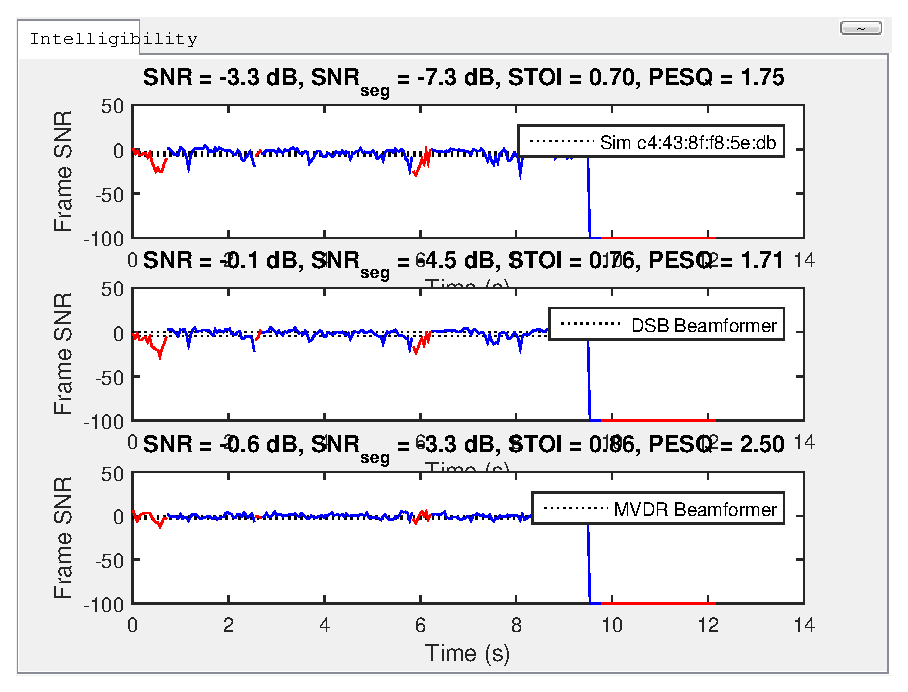
\includegraphics[scale = 0.88] {Screenshots_simulatie/Intelligibility/Simulatie6} % l b r t]
	\caption[Intelligibility simulation 6]{Intelligibility simulation 6: With reverberations, White noise added at 60dB SNR, with position errors with a sigma of $0.05 cm$} 
	\label{fig:Isim6}
\end{figure}
\FloatBarrier
\section{Office room experiments}
\label{app:room}
\FloatBarrier

\subsection{Office room experiment 1}
\label{app:room1}

\begin{figure}[h!]
	\centering  
	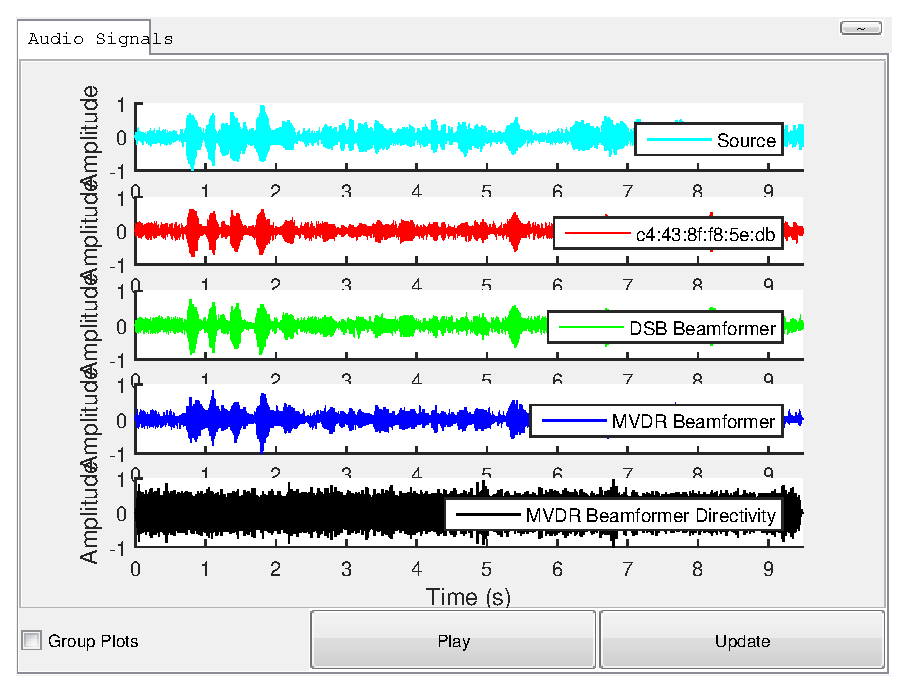
\includegraphics[scale = 0.88] {Screenshots_experimenten/Audio_signals/signals_18u36} % l b r t]
	\caption[Audio signals office room experiment 1]{Audio signals office room experiment 1: With an interfering audio source, $\theta = -90\degree$} 
	\label{fig:Aroom1}
\end{figure}

\begin{figure}[b!]
	\centering  
	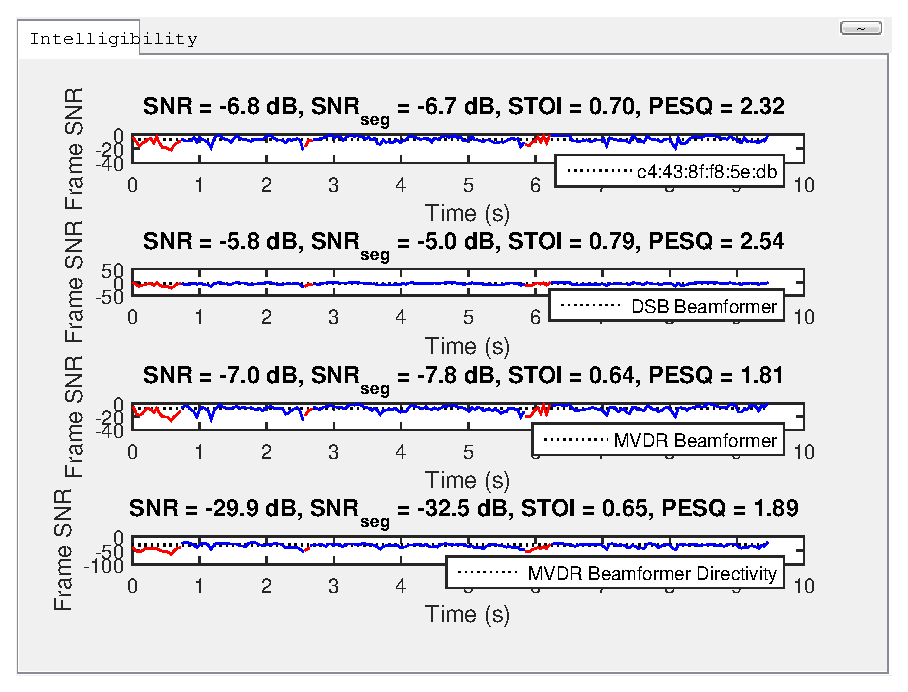
\includegraphics[scale = 0.88] {Screenshots_experimenten/Intelligibility/Intelligibility_18u36} % l b r t]
	\caption[Intelligibility office room experiment 1]{Intelligibility office room experiment 1: With an interfering audio source, $\theta = -90\degree$} 
	\label{fig:Iroom1}
\end{figure}

\FloatBarrier

\subsection{Office room experiment 2}
\label{app:room2}

\begin{figure}[h!]
	\centering  
	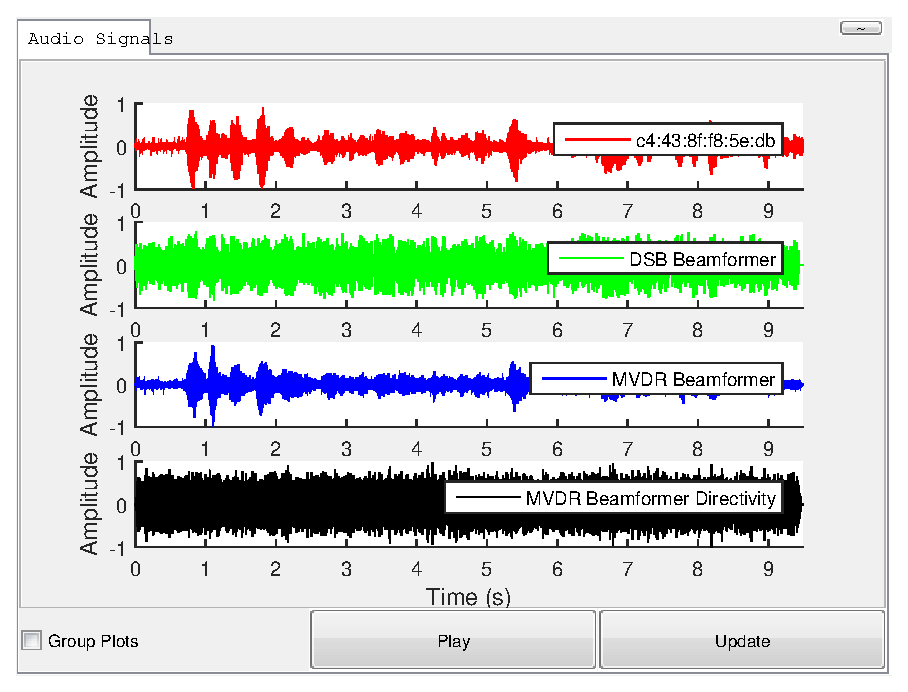
\includegraphics[scale = 0.9] {Screenshots_experimenten/Audio_signals/signals_20u21} % l b r t]
	\caption[Audio signals office room experiment 2]{Audio signals office room experiment 2: With an interfering audio source, $\theta = 0\degree$} 
	\label{fig:Aroom2}
\end{figure}

\begin{figure}[b!]
	\centering  
	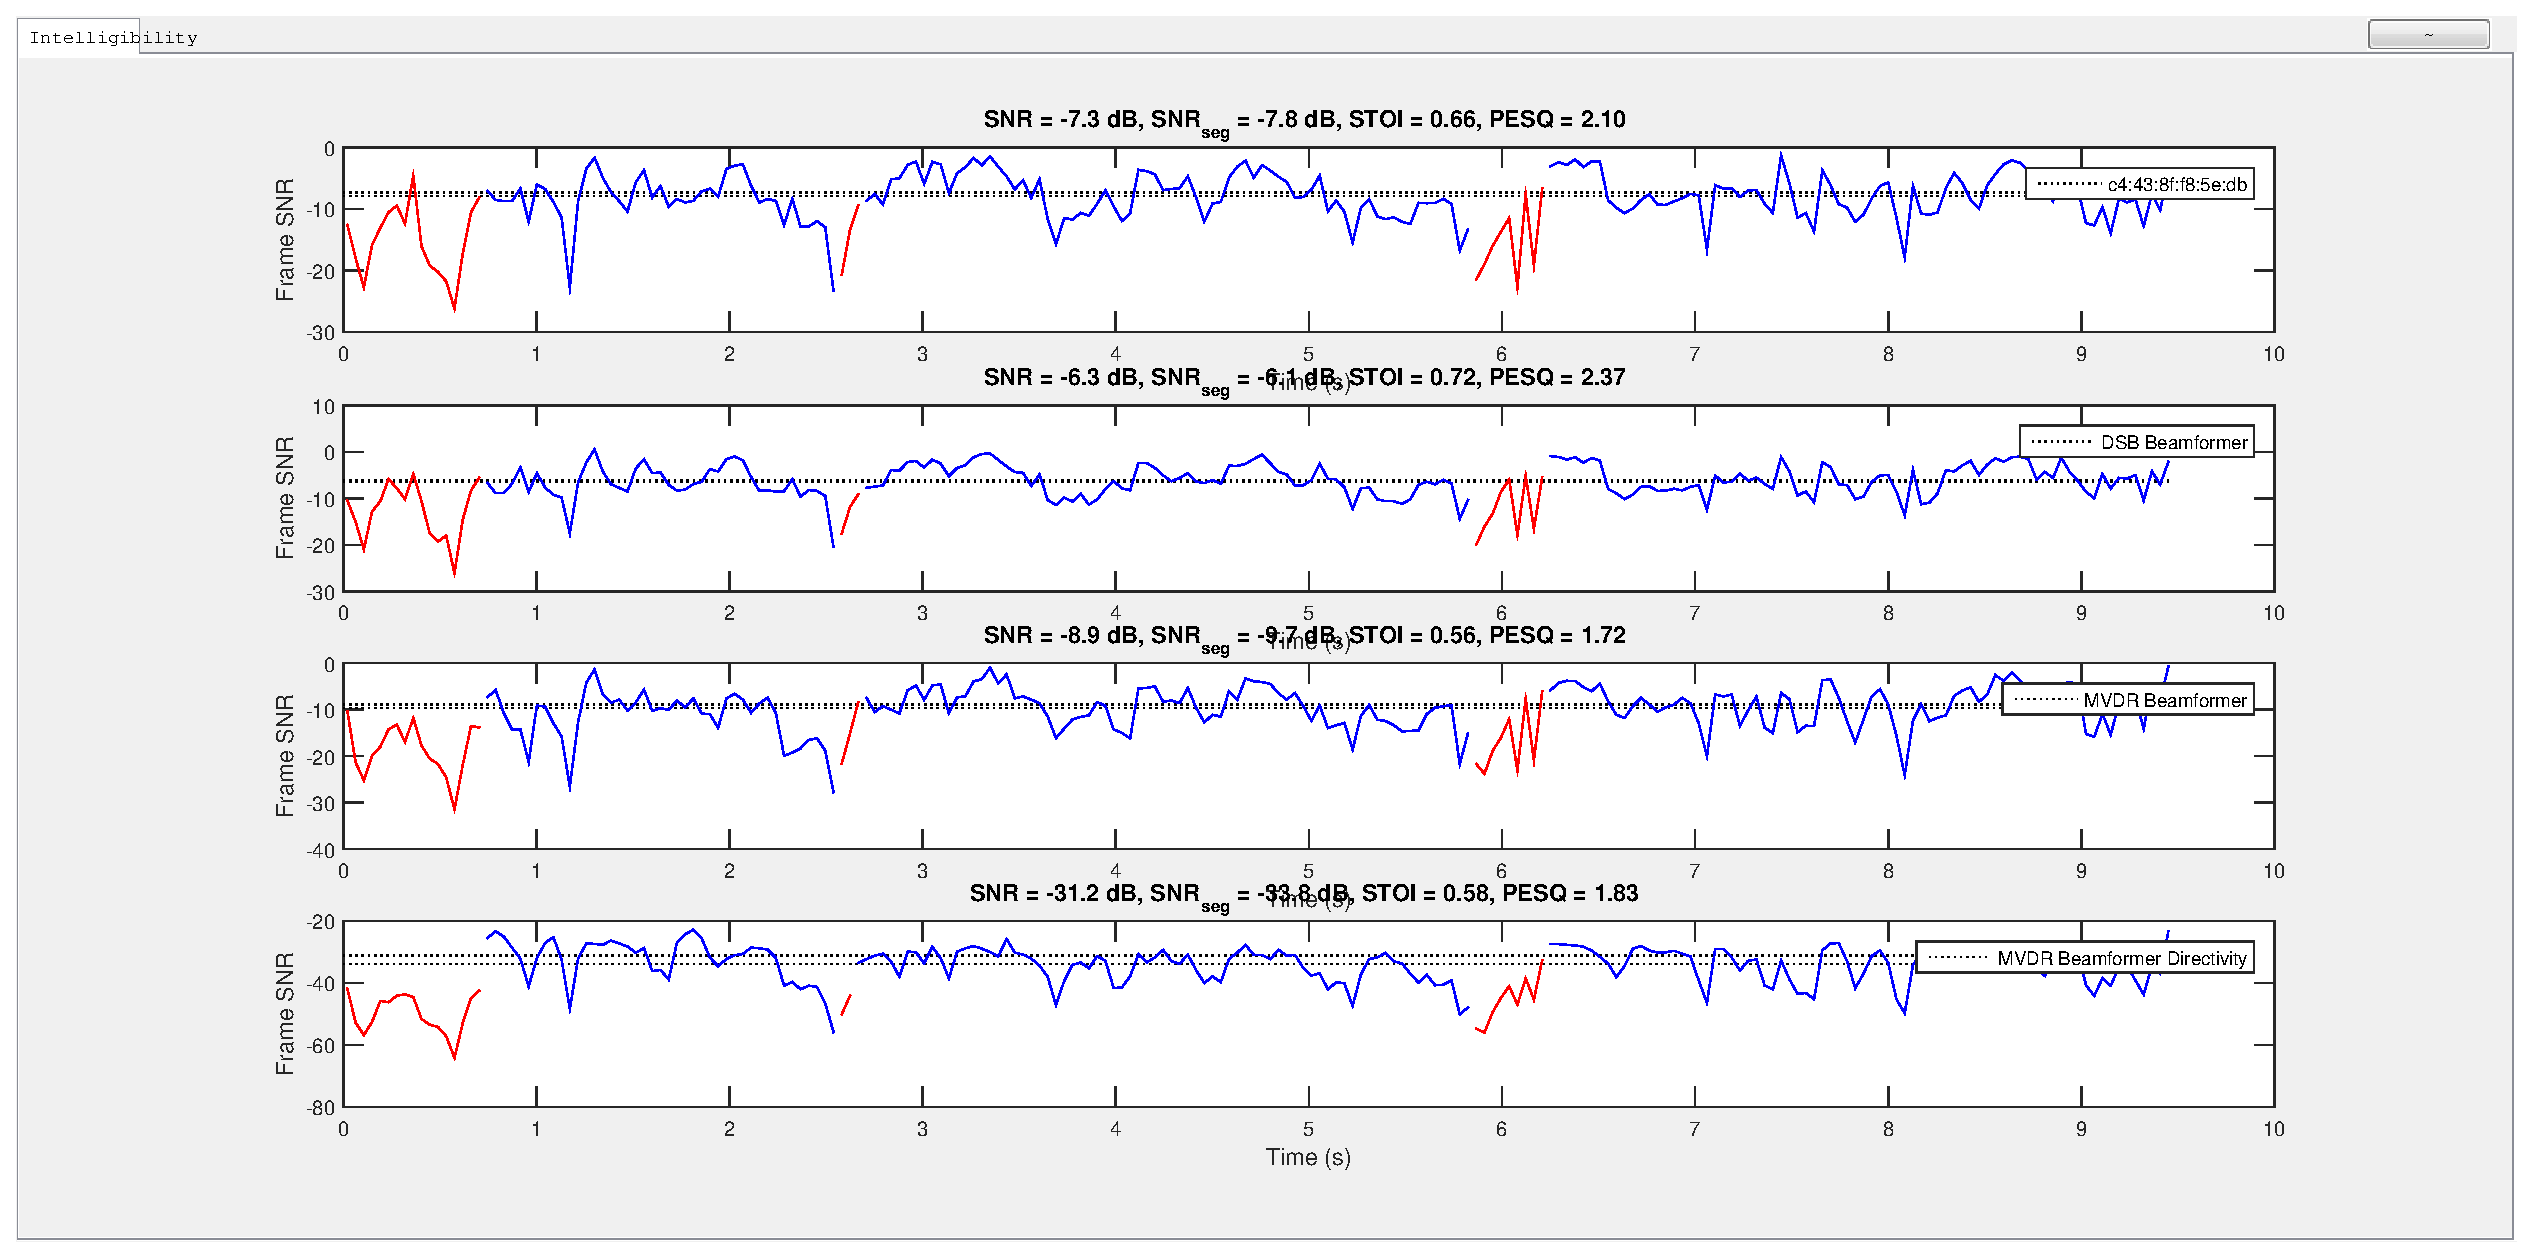
\includegraphics[width = \columnwidth] {Screenshots_experimenten/Intelligibility/Intelligibility_20u21} % l b r t]
	\caption[Intelligibility office room experiment 2]{Intelligibility office room experiment 2: With an interfering audio source, $\theta = 0\degree$} 
	\label{fig:Iroom2}
\end{figure}

\FloatBarrier

\subsection{Office room experiment 3}
\label{app:room3}

\begin{figure}[h!]
	\centering  
	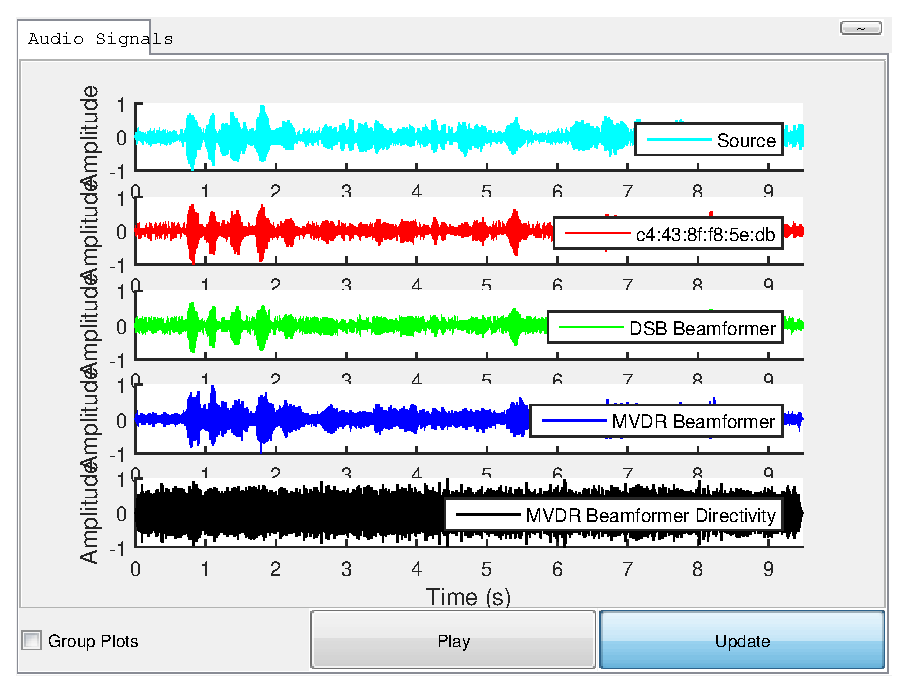
\includegraphics[scale = 0.9] {Screenshots_experimenten/Audio_signals/signals_20u29} % l b r t]
	\caption[Audio signals office room experiment 3]{Audio signals office room experiment 3: With an interfering audio source, $\theta = 90\degree$} 
	\label{fig:Aroom3}
\end{figure}

\begin{figure}[b!]
	\centering  
	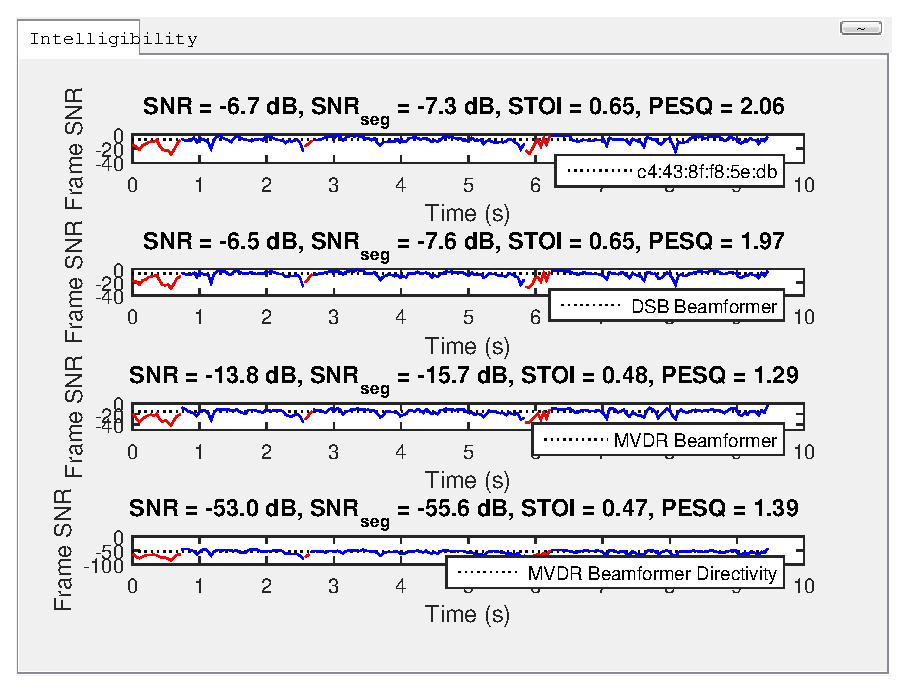
\includegraphics[scale = 0.9] {Screenshots_experimenten/Intelligibility/Intelligibility_20u39} % l b r t]
	\caption[Intelligibility office room experiment 3]{Intelligibility office room experiment 3: With an interfering audio source, $\theta = 90\degree$} 
	\label{fig:Iroom3}
\end{figure}

\FloatBarrier

\subsection{Office room experiment 4}
\label{app:room4}

\begin{figure}[h!]
	\centering  
	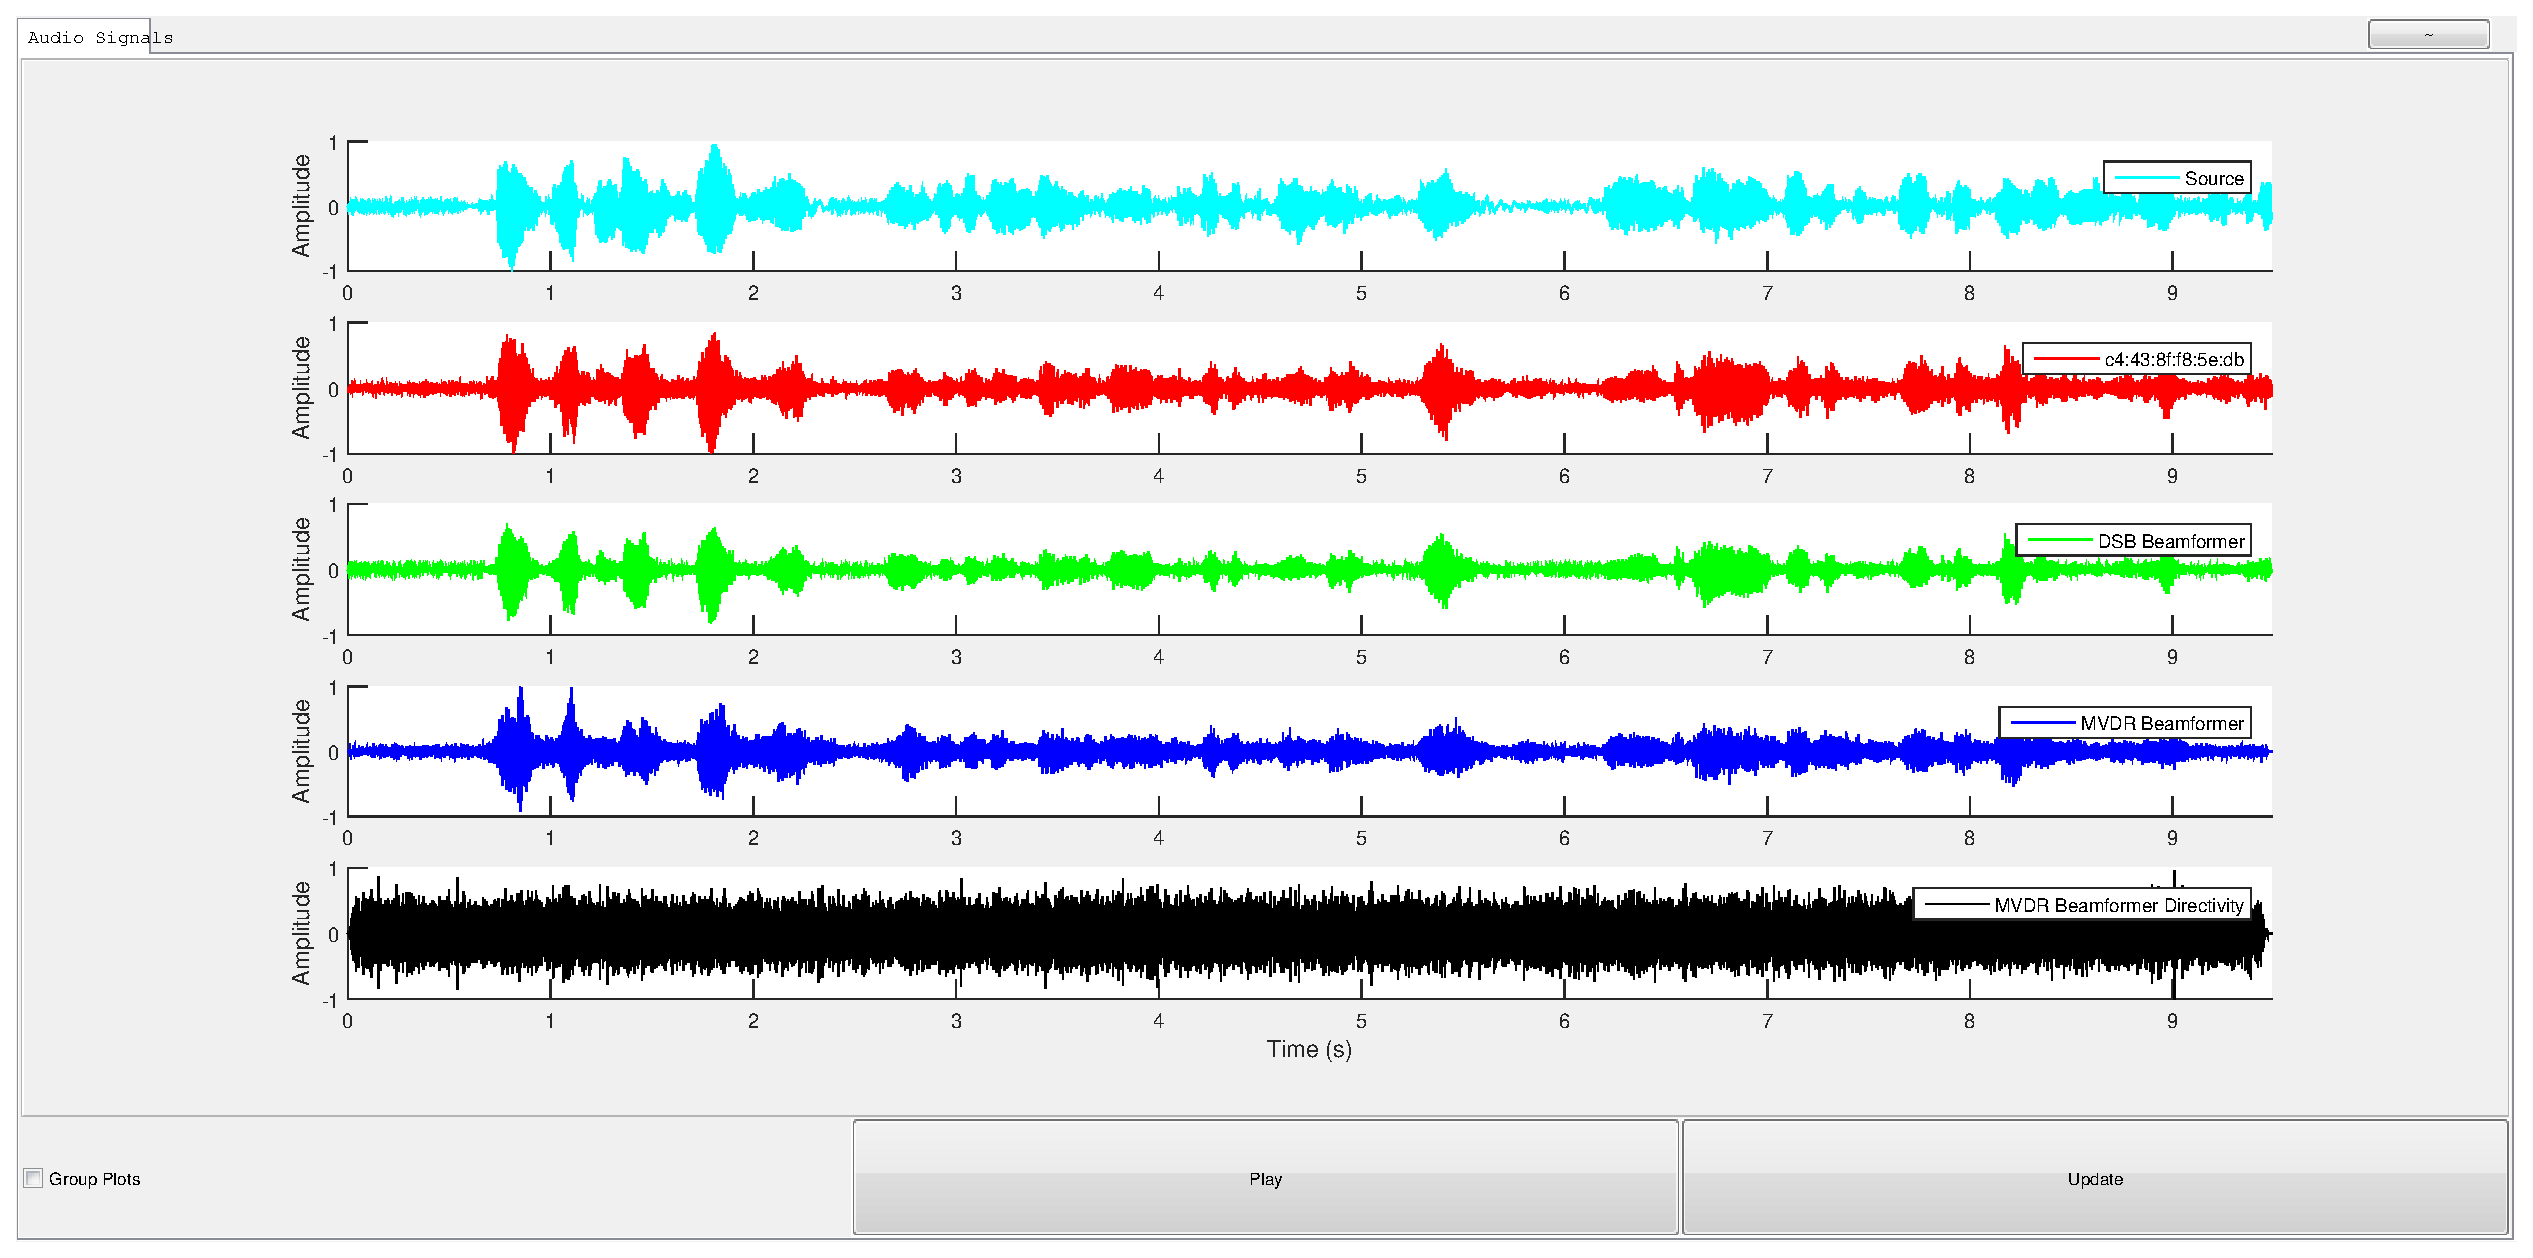
\includegraphics[width = \columnwidth] {Screenshots_experimenten/Audio_signals/signals_20u55} % l b r t]
	\caption[Audio signals office room experiment 4]{Audio signals office room experiment 4: With an interfering audio source, Different orientations} 
	\label{fig:Aroom4}
\end{figure}

\begin{figure}[b!]
	\centering  
	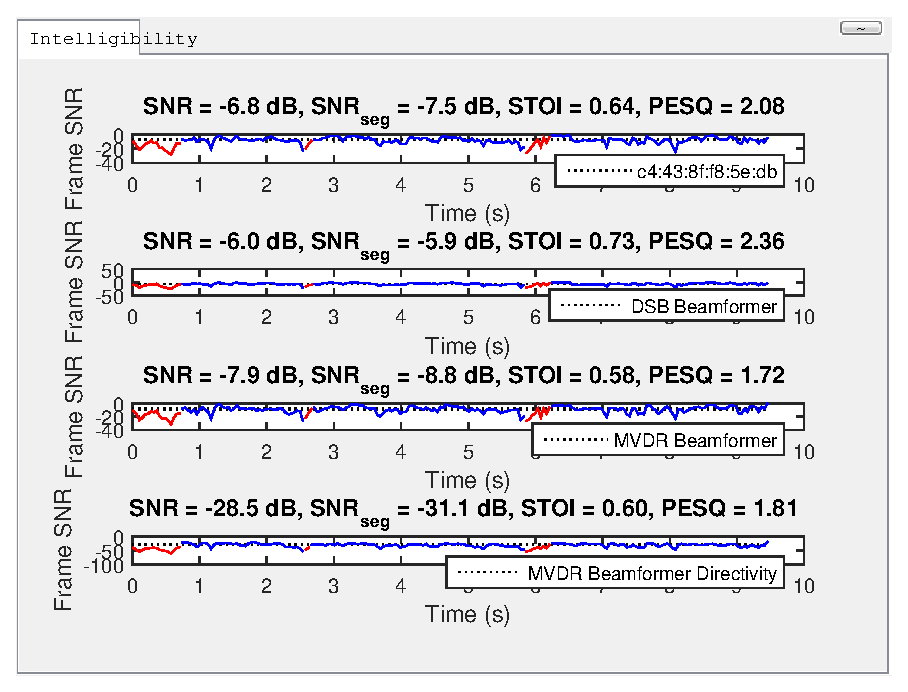
\includegraphics[scale = 0.9] {Screenshots_experimenten/Intelligibility/Intelligibility_20u55} % l b r t]
	\caption[Intelligibility office room experiment 4]{Intelligibility office room experiment 4: With an interfering audio source, Different orientations} 
	\label{fig:Iroom4}
\end{figure}

\FloatBarrier

\subsection{Office room experiment 5}
\label{app:room5}

\begin{figure}[h!]
	\centering  
	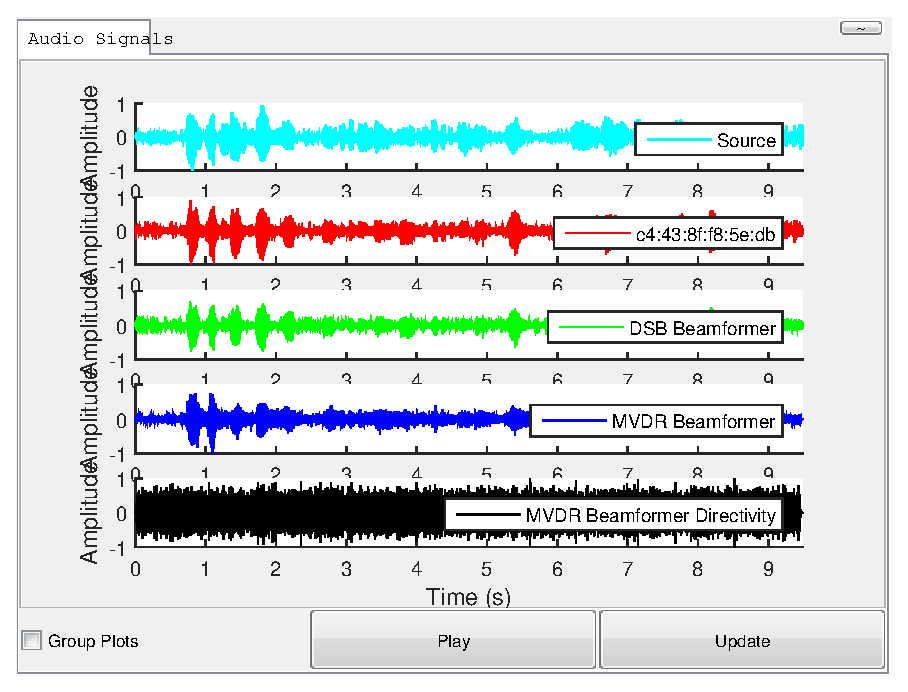
\includegraphics[scale = 0.9] {Screenshots_experimenten/Audio_signals/signals_21u07} % l b r t]
	\caption[Audio signals office room experiment 5]{Audio signals office room experiment 5: With an interfering audio source, Linear array} 
	\label{fig:Aroom5}
\end{figure}

\begin{figure}[b!]
	\centering  
	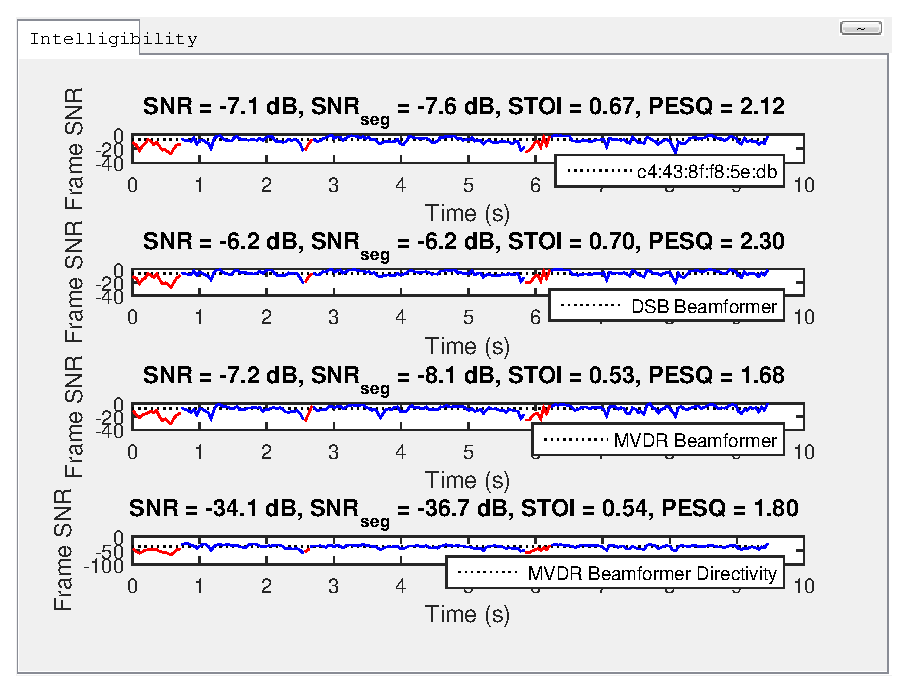
\includegraphics[scale = 0.9] {Screenshots_experimenten/Intelligibility/Intelligibility_21u07} % l b r t]
	\caption[Intelligibility office room experiment 5]{Intelligibility office room experiment 5: With an interfering audio source, Linear array} 
	\label{fig:Iroom5}
\end{figure}

\FloatBarrier

\section{Anechoic chamber experiments}
\label{app:anechoic}

\subsection{Anechoic chamber experiment 1}
\label{app:anechoic1}

\FloatBarrier

\begin{figure}[h!]
	\centering  
	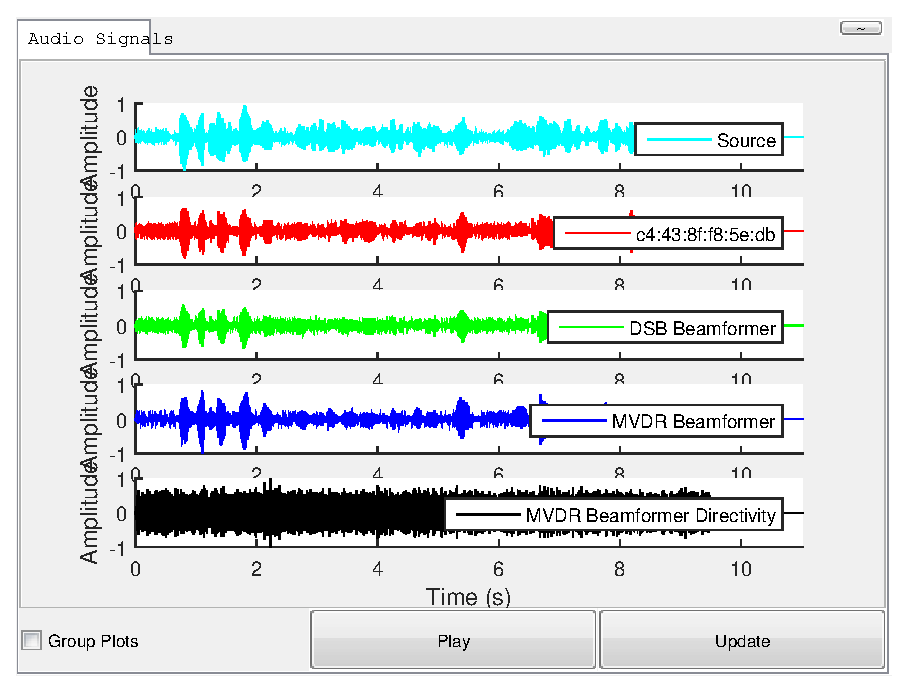
\includegraphics[scale = 0.85] {Screenshots_experimenten/Audio_signals/signals_18u27} % l b r t]
	\caption[Audio signals anechoic chamber experiment 1]{Audio signals anechoic chamber experiment 1: With an interfering audio source} 
	\label{fig:Aanechoic1}
\end{figure}

\begin{figure}[b!]
	\centering  
	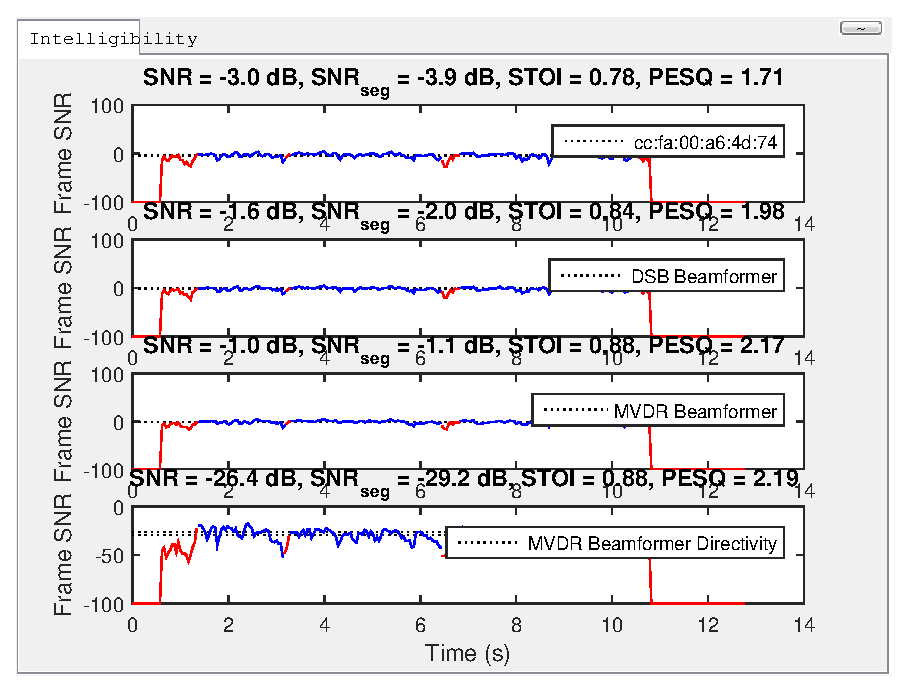
\includegraphics[scale = 0.85] {Screenshots_experimenten/Intelligibility/anechoic} % l b r t]
	\caption[Intelligibility anechoic chamber experiment 1]{Intelligibility anechoic chamber experiment 1: With an interfering audio source} 
	\label{fig:Ianechoic1}
\end{figure}

\FloatBarrier